\documentclass[11pt,oneside,reqno]{amsart}
\usepackage{caption}
\usepackage{graphicx}
\usepackage{pict2e}
\usepackage{amssymb}
\usepackage{amsthm}                % better theorem environments
\usepackage[margin=1in]{geometry}  % set the margins to 1in on all sides
\usepackage{graphics}
\usepackage{epstopdf}
\usepackage{amsmath}
\usepackage{graphicx}
\usepackage{subfigure}
\usepackage{latexsym}
\usepackage{amsmath}
\usepackage{amsfonts}
\usepackage{amssymb}
\usepackage{tikz}
\usepackage{mathdots}
\usepackage{mathtools}
\usepackage{hyperref}
\usepackage{comment}
\usepackage{mathtools}
\usepackage{float}
\usepackage[mathscr]{euscript}



\usepackage{epsfig}  	
\newtheorem{thm}{Theorem}[section]
\newtheorem{prop}[thm]{Proposition}
\newtheorem{lem}[thm]{Lemma}
\newtheorem{cor}[thm]{Corollary}

\theoremstyle{definition}
\newtheorem{theorem}{Theorem}[section]
\newtheorem{lemma}[theorem]{Lemma}
\newtheorem{corollary}[theorem]{Corollary}
\newtheorem{proposition}[theorem]{Proposition}
\newtheorem{noname}[theorem]{}
\newtheorem{sublemma}{}[theorem]
\newtheorem{conjecture}[theorem]{Conjecture}
\newtheorem{summary}[theorem]{Summary}
\theoremstyle{definition}
\newtheorem{definition}[theorem]{Definition}
\newtheorem{example}[theorem]{Example}
\theoremstyle{remark}
\newtheorem{remark}[theorem]{Remark}
\numberwithin{equation}{section}
\newcommand{\ba}{\backslash}
\bibliographystyle{alphanum} 

\numberwithin{equation}{section}
\newcommand{\R}{\mathbf{R}}  % The real numbers.

\usepackage{fancyhdr} % Headers and footers
\usepackage{lastpage}
\pagestyle{fancy} % All pages have headers and footers
\fancyhead{} % Blank out the default header
\fancyfoot{} % Blank out the default footer
\fancyhead[L]{Spam Email Classification Using Machine Learning} % Custom header text
\fancyhead[R]{\today} % Custom header text
\fancyfoot[R]{Page \thepage \  of \pageref{LastPage}} % Custom footer text

\begin{document}
\raggedbottom

\title{Spam Email Classification Using Machine Learning}

\author{Imaad Ahmed}
\address{Department of Computer Science, Louisiana State University, 
Baton Rouge, LA 70803 USA}
\email{imaadahmed19@gmail.com}
\author{Zahra Khatami}
\address{Department of Electrical Engineering, Louisiana State University, 
Baton Rouge, LA 70803 USA}
\email{z.khatami88@gmail.com}
\author{Mustafa Hajij}
\address{Department of Mathematics, Louisiana State University, 
Baton Rouge, LA 70803 USA}
\email{mhajij1@math.lsu.edu}

\author{Ali Moharrer}
\address{Department of Electrical Engineering, Louisiana State University, 
Baton Rouge, LA 70803 USA}
\email{alimoharrer@gmail.com}
\author{Brandon Oubre}
\address{Department of Computer Science, Louisiana State University, 
Baton Rouge, LA 70803 USA}
\email{br.oubre@yahoo.com}


%%%
%%% The following is for the abstract.  The abstract is optional and
%%% if not used just delete, or comment out, the following.
%%%
\begin{abstract}
Spam e-emails are becoming a major problem on the internet and the need for an automatic spam filter is a necessity. In this paper we use machine learning to address the spam classification problem. By comparing the performance of a variety of classifiers, we have determined which techniques are particularly well suited for this task. Our analysis of the classifiers also reveals some interesting properties about the nature of spam emails that can be used in the further development of effective spam classification systems. 
\end{abstract}


\keywords{} 

\maketitle

\thispagestyle{fancy} % All pages have headers and footers

\section{Introduction}
Spam e-mails are a major problem on the internet, with millions of copies of unwanted emails being sent to email users every second. Spam emails contain no useful information and are a waste of memory storage and processing time. Moreover, spam emails may compromise personal or confidential information and even the security of operating systems. The need for a program or a service that detects spam emails and take the proper actions is clear and demanding, as evidenced by the adoption of spam classification systems by every major email service. Although there are many services that provide spam filtering, there are still many challenges in this regard.

In this report we use machine learning to address this problem. Spam detection can be regarded as a classification problem: classify each received email as a spam email or as a legitimate one. This email classification problem is not a trivial one for multiple reasons. For instance, most of the spam emails contain many common keywords also used in legitimate emails. Moreover, there is no class of keywords that is specific only to spam. Even the most common spam keywords such as "money", "$\$$", or "free" may occur in legitimate emails. A legitimate email that is received from a bank often contains these keywords, and one clearly does not want to classify such emails as spam. Hence many correlated features should be addressed and studied simultaneously in order to classify emails successfully.

There are many data mining techniques that can take care of the aforementioned problems. Here we want to examine a few of the most known techniques in Machine Learning to construct a classifier with competitive performance. The performance should account for low error rates, a small number of false positives (the number of legitimate emails that are classified as spam), and a fast convergence time (lower training time). Note that the number of false positives is an important measure of the performance of our classifier since the cost of classifying an important legitimate emails as a spam is high for a spam filter's end users.

Our method to study the classification problem is by comparing several classification models. In our study we used Bayes Networks, Naive Bayes Classifiers, ANNs (Artificial Neural Networks), SVM (Support Vector Machine), C4.5 (Decision Trees), Bagging (Bootstrap Aggregating) on decision trees and AdaBoost (Adaptive Boost) on decision stumps. In our implementations we used three programming languages : \textbf{R}, \textbf{Python}, and \textbf{Java}. For the SVM implementation we used Scikit-learn is a Python \cite{scikit-learn}.

\section{Choosing The Data Set}

In our classification study we used a spam database available at the UCI Machine Learning repository \cite{spam}. There are a total of $57$ continuous attributes (features) in this data set. These features are either $(1)$ the frequency of certain keywords, $(2)$ the frequency of specific characters, or $(3)$ the average run length of a string of capitals. The total number of instances in this data set is $4601$, which all are labeled as either spam ($1$) or legitimate ($0$). The output is placed on the $58^{th}$ column of the data set.

We chose to use this data set because it was freely available and well-studied. Additionally, the data set has already decided which keywords and special characters to include as features. This saved us from having to determine which features of an email to consider in our classification task and allowed us to instead focus on comparing the performance of various techniques. A downside of this data set, however, is that by not having access to the raw data we were unable to apply certain techniques such as TF-IDF (Term Frequency - Inverse Document Frequency). Despite this drawback, we were still able to identify several well-performing classification models.


\section{Overview of The Method Of Classification}
In this section we give an overview of most of the methods that we used in our email classification task. We give a complete analysis of every classifier in the results and conclusion sections.
\subsection{Artificial Neural Networks}

In this section we show how to use artificial neural networks (ANNs) for our email classification problem. Our ANN can be seen as a series of layers, with each layer containing one or mode neurons. A linear combination of inputs is fed to the second layer, which is the first hidden layer. Similar to the input layer, the values of hidden layers are fed to the next layer, and the same procedure continues until we reach the output layer. Generally, ANNs may have multiple hidden layers. However, it has been shown in many situations that multiple hidden layers can result in over-fitting. For our approach we decided that our network should consist of a single hidden layer.

\subsubsection{Training Phase}
Since many features in our data set may not be useful for classification, we perform feature selection on our data set in order to speed the classification learning process. In particular, we use the information gain ratio to measure the degree of importance for each feature. Recall that the information gain is given by \ref{eq:infogain}.
\begin{align} \label{eq:infogain}
InfoGain(X_i) = \dfrac{I(X_i;Y)}{H(X_i)},
\end{align}
where $H(X_i)$ is the entropy corresponding to feature $X_i$, and $I(X_i;Y)$ is the mutual information between the feature $X_i$ and the output. Observe here that information gain metric accounts for those situations where the feature can perfectly divide the output into objective classes. For example, consider a particular feature that can take many values, it is probable that it may perfectly divide data, and result in higher splitting criterion, while this feature might be totally irrelevant and not important. However, information gain ratio prevents such situations by putting the entropy in the denominator.

From the set of $57$ features, we extracted $10$ features with the highest information gain values. We found that features are \textbf{``Remove", ``Free", ``Your", ``000", ``Money", ``hp", ``hp1", ``George", ``!", and ``$\$$"}. Note that the keywords such as ``Free", ``Money" or ``$\$$" can be found in most spam emails.

After pre-processing the data, we use the processed data from these $10$ inputs to train the neural network. In our implementation, we use \textit{neuralnet} package \cite{neuralnet}, which is in the \textbf{R} programming language. We choose $1$ hidden layer to train the network. We find that $1$ hidden layer results in a really high accuracy and at the same time it avoids the over-fitting problem that can result by adding more hidden layers. The optimal number of hidden nodes is chosen by a $10$-fold cross validation over the data set. In particular we set the possible number of hidden nodes to be inclusively between $1$ and $10$. We chose this range because the optimal number of hidden nodes is often between the number of input nodes and the number of output nodes, which in our case is 10 and 1 respectively. It turns out that a neural network with $8$ hidden nodes has the best accuracy among all possible cases for our data. Figure \ref{NN} shows the overall trained network for the email classification as well as the weights of the edges in the network.

\begin{figure}[H]
  \centering
   {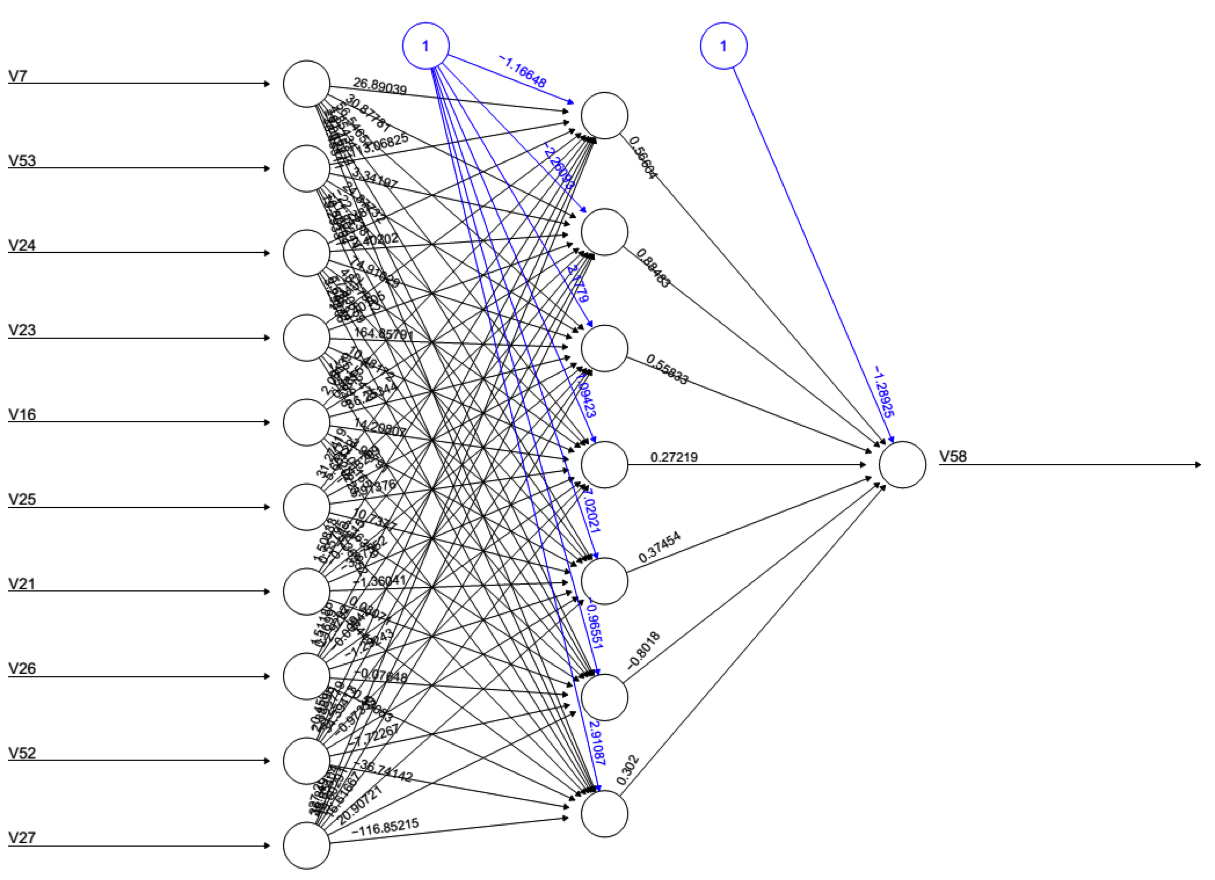
\includegraphics[keepaspectratio=true, width=.95\textwidth]{NN}
   \caption{The trained ANN with $8$ hidden nodes and optimized using $10$-fold cross-validation}
  \label{NN}}
\end{figure}

% NOTE: Took out testing ANN section because it belongs in the results section. The same info is contained there.

\subsection{Support Vector Machine}
Support Vector Machine is a supervised machine-learning method that has been used for classification and regression analysis. The linear vector machine algorithm takes as an input a data consists of training examples $(x_1,y_1),...,(x_N,y_N)$ where $x_i\in \mathbb{R}^p$ and $y_i\in{-1,+1}$ and return an $p-1$ hypersurface, also called the decision boundary surface, that best separate the data points $x_1,...x_N$ according to their labeling. In the case where the decision surface is a $p-1$ hyperplane then we have a linear support vector machine. For the sake of illustration we present  the idea of linear support vector machine here.
\subsubsection{Linear Support Vector Machine}
Let $\mathcal{D}=\{(x_i,y_i)\in \mathbb{R}^p\times \{-1,+1\} ,i\in \{1,..,N\} \}$. We want to find the $p-1$ hyperplane that best linearly separate the points $x_1,...,x_N$ according to their labeling. Any $p-1$ hyperplane in $\mathbb{R}^p$ has the form :\
\begin{equation}
\label{plane}
<w,x>=b
\end{equation}   
where <,> is the Euclidean inner product, $w\in \mathbb{R}^p$ and $b\in \mathbb{R}$. Hence the problem is to find the best $w$ and $b$ that best separate the data points. Equation \ref{plane} can be written as $<w,x>-b=0$. Now we want to choose $w$ and $b$ such that for all $x_i$ such that $y_i=1$ we have
\begin{equation}
\label{cond1}
<w,x_i>-b \geq 1
\end{equation}
and
\begin{equation}
\label{cond2}
<w,x_i>-b \leq -1
\end{equation}  
on all the points $x_i$ such that $y_i=-1$. The distance between the plane $<w,x>-b=1$ and $<w,x>-b=1$ is $\frac{2}{||w||}$ and hence the best choice of the plane $\ref{plane}$ is the plane the maximizes the distance $\frac{2}{||w||}$ subject to conditions $\ref{cond1}$ and $\ref{cond2}$ or equivalently it is the plane the minimizes $||w||$ subject to:
\begin{equation}
y_i(<w,x_i>-b) \leq -1
\end{equation} 
for $i \in {1,...,N}$.
\begin{example}
Suppose that we have 2 features in our data set and we want to classify the elements shown in Figure \ref{SVM_1}. We can see that we have the class of squares and the class of the circles.
\begin{figure}[H]
  \centering
   {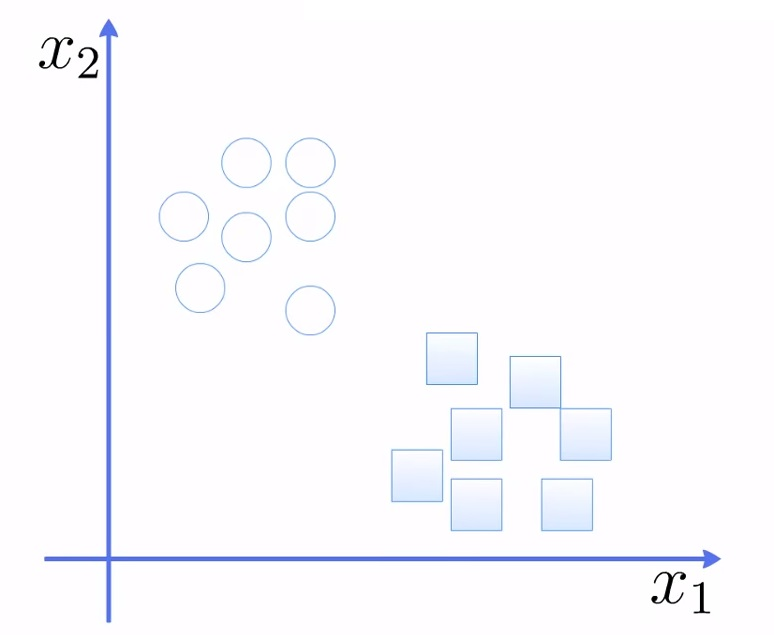
\includegraphics[scale=0.2]{SVM_1}
   \caption{The data set}
  \label{SVM_1}}
\end{figure}
The goal of SVM is to find a hyperplane, the green line in Figure \ref{SVM_2} that best separate the set of squares and the set of circles.
\begin{figure}[H]
  \centering
   {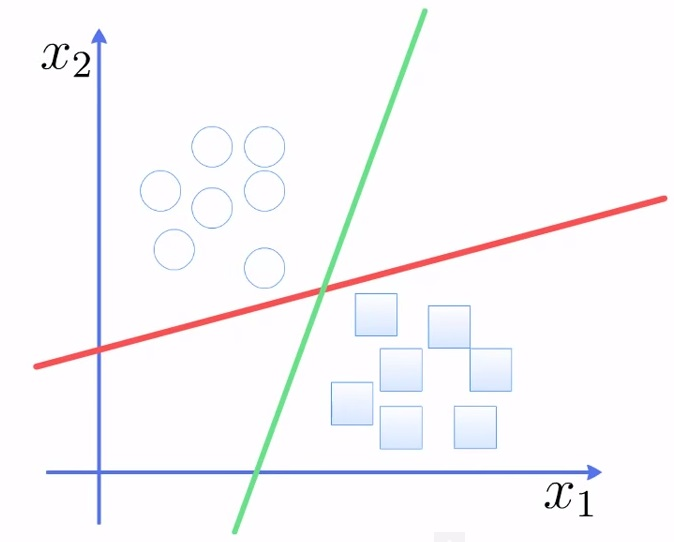
\includegraphics[scale=0.2]{SVM_2}
   \caption{Using linear SVM to separate the data into two classes}
  \label{SVM_2}}
\end{figure}
\end{example}
\subsubsection{The Kernel Trick}
The dot product in \ref{plane} can be replaced by a nonlinear \textit{kernel function}. A kernel is a map $k:\mathcal{X}\times \mathcal{X}\longrightarrow \mathbb{R}$ where $\mathcal{X}$ is the input space. Intuitively, the value $k(x_i,x_j)$ measures a kind of similarity between the data point $x_i$ and $x_j$. Some common kernels:
\begin{enumerate}
\item The Gaussian radial basis kernel: $k(x_i,x_j)=e^{-\alpha ||x_i-x_j||^2}$ where $\alpha>0$ is a parameter
\item The sigmoid kernel: $k(x_i,x_j)=\tanh (\alpha <x_i,x_j>+r)$ where $r<0$ and $\alpha>0$. 
\end{enumerate}   
\subsection{AdaBoost}
AdaBoost is a technique to create a sequence of an increasingly complex classifiers out of multiple simple classifiers. In this model we start by learning a very simple classifier and then evaluate its errors and then focus the next predictor on getting these examples right. This procedure tends to discover the examples that are difficult to predict and focuses later classifiers on better predicting these examples. In the end we combine the entire set of classifiers using some weighted combination to obtain a powerful classifier. In this method each individual learner tends to be very simple and by combining  many of these simple predictor we are able to learn a complex function. For our implementation of AdaBoost on decision stumps, we used the Weka Java Library \cite{Weka}.
\subsubsection{Illustrative Example} 
Suppose that we have the data set $D_1$ illustrated in Figure \ref{adaboost}. Observe that the data set has some $+1$ entries in red and some $-1$ entries in blue. We want to classify the data but we want to restrict ourselves to very simple classier. So in this example we will restrict ourselves to one level decision tree, also known as a decision stump.


\begin{figure}[H]
  \centering
   {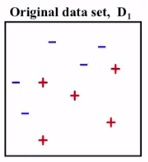
\includegraphics[scale=0.8]{boosting_1}
   \caption{The data set $D_1$}
  \label{adaboost}}
\end{figure}
In the first step we show the how the simple classifier learns to classifier the examples as shown in Figure \ref{adaboost1}. We observe that this classifier succeeds at obtaining most of the most correctly. 
\begin{figure}[H]
  \centering
   {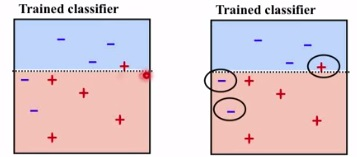
\includegraphics[scale=0.8]{boosting_2}
   \caption{The simple classifier succeeds at classify most of the example. The examples that are not classified correctly will be focused on in the second step }
  \label{adaboost1}}
\end{figure}
We will focus in the next step on the examples that were not classified correctly on the first step. In the second step we increase the weight (our desire to correctly classify) of the these points. Now we have a new data set $D_2$ which consists the original data set $D_1$ but now we have weights assigned to the points. This weight is indicated visually by the size of the sign in Figure \ref{adaboost2}.
\begin{figure}[H]
  \centering
   {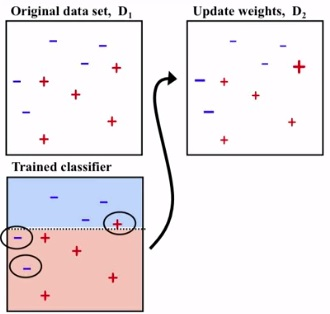
\includegraphics[scale=0.8]{boosting_3}
   \caption{Contracting the data set $D_2$ in order to classify the examples that were classified wrong by the previous classifier}
  \label{adaboost2}}
\end{figure}
We now train the second classifier and we focus on these highly weighted points and obtain the classified set shown in Figure \ref{adaboost3}
\begin{figure}[H]
  \centering
   {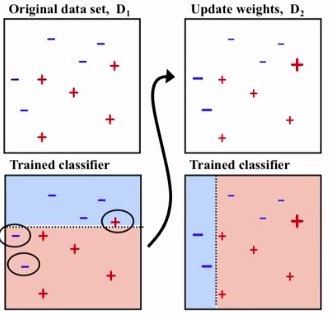
\includegraphics[scale=0.8]{boosting_4}
   \caption{Using the second classifier to classify the examples that we fail to classify by the first classifier}
  \label{adaboost3}}
\end{figure}
We repeat this process again the examples that were classified wrong by the first two classifiers as shown in Figure \ref{adaboost4}.
\begin{figure}[H]
  \centering
   {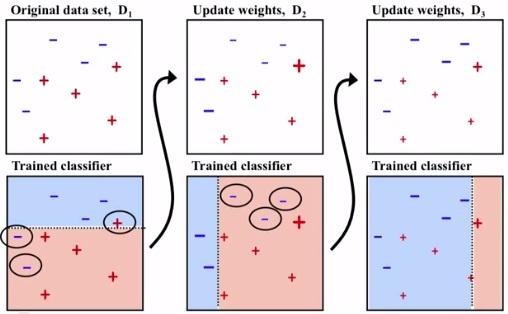
\includegraphics[scale=0.8]{boosting_5}
   \caption{Using the third classifier to classify the examples that we failed to classify in the first two classifiers}
  \label{adaboost4}}
\end{figure}
In the end each of these classifiers is assigned a weight and their weighted combination is our complex predictor. See Figure \ref{adaboost5}
\begin{figure}[H]
  \centering
   {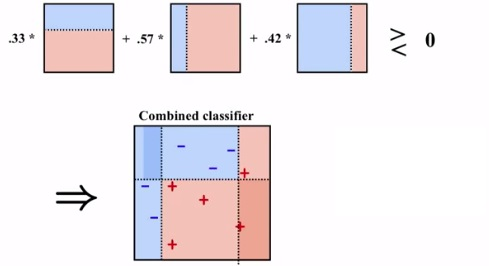
\includegraphics[scale=0.8]{boosting_6}
   \caption{Obtaining the final complex classifier as a weighted combination of the simple classifiers}
  \label{adaboost5}}
\end{figure}
\subsection{Bagging}
Bagging stands for bootstrap aggregation, and was implemented in Java using Weka \cite{Weka}. Bagging is a technique for learning many classifiers, each using only a portion of the data, and then combining these classifiers with some averaging technique. The idea behind bagging is to reduce the overfitting of a class of models. Recall that we overfit when we "memorize" the data set and obtain a lower training error on that training data set than what we would see on a validation data. The idea behind bagging is similar to the idea of splitting in that of the cross validation. The difference is that in bagging we split data for a better classification versus testing in cross validation.


We briefly explain how bagging works. We take a collection of $N$ data points and we generate a new data set $N^{\prime}$ by simply randomly drawing these $N^{\prime}$ data points from the original data set with replacement. Bagging then creates a $K$ learners. Each learner is created independently and generates its own data set by drawing $N^{\prime}$ data points from the original data with replacement. It then trains a classifier for each one of these data sets and when we test we take all of these all predictors and we combine their results with an unweighted combination.

\subsection{C4.5 Decision Trees and Naive Bayes Classifier}
Both the C4.5 decision tree algorithm and the Naive Bayes classifier were implemented in Java using the Weka library \cite{Weka}. In the Weka library the C4.5 algorithm is referred to as J48. C4.5 is similar to the classic ID3 algorithm, uses information gain as a splitting criterion, handles continuous attributes, and conducts post-pruning. The Weka implementation of Naive Bayes also handles continuous attributes. These algorithms work similarly as what we described in class and we use them as a baseline for comparison with other classifiers.

\subsection{Bayes Network}
We implemented the Bayes Network classifier using the Weka library in Java \cite{Weka}. The reason that we decided to use a Bayes Network is for comparison with the Naive Bayes Classifier, since a Bayes Network takes conditional independence relations between attributes into account. An interesting feature of the Weka Bayes Network implementation is that it uses hill climbing algorithms, such as K2 and B, along with general algorithms, such as simulated annealing and tabu search, in order to learn the conditional independence relations amongst attributes. This means that we do not need to consult an expert or make an educated guess in order to decide on the Bayes Network topology. Instead we let the library learn the network topology from the data. This approach allows us to effectively compare the result of the Naive Bayes Classifier and the Bayes Network.

\section{Results}
To compare the effectiveness of the classifiers on our data, we ran 10-fold cross validation on the data set using each classifier and then compared three main results of the cross validation: overall accuracy, the number of legitimate emails classified as spam (false positives), and the runtime in seconds. These results are displayed in Table \ref{table:results}.
\begin{table}[H]
\centering
\begin{tabular}{r | r r r r}
	Classifier & Accuracy & 95\% Conf. & False Positives & Runtime (s) \\ \hline
	Naive Bayes & 79.6131\% &\(\pm\) 1.1641\%& 858 & 0.561\\
	Bayes Net & 89.6066\% &\(\pm\) 0.8818\%& 168 & 1.438\\
	AdaBoost & 89.9587\% &\(\pm\) 0.8684\%& 215 & 3.853\\
	ANN & 91.6739\% &\(\pm\) 0.7983\%& 155 & \(>\)60.0\\
	SVM & 92.1565\% &\(\pm\) 0.7768\%& 66 & 0.588\\
	C4.5 & 92.6972\% &\(\pm\) 0.7518\%& 152 & 4.118\\
	Bagging & 94.0665\% & \(\pm\) 0.6826\% & 110 & 12.496
\end{tabular}
\caption{Classifier results from 10-fold cross validation.}
\label{table:results}
\end{table}
\begin{description}
	\item[Accuracy] The overall accuracy of the classifier is the percent of data points in the test partition that a trained classifier correctly predicted. This result is important for comparison because a classifier with a higher accuracy performed more correct predictions over the entire test partition than a classifier with a lower accuracy.
	\item[95\% Confidence Margin] Let \(A\) be the observed accuracy of a classifier and \(N=4601\) be the number of examples in our data set. We calculate \(\sigma = \sqrt{\frac{A(1-A)}{N}}\) and calculate that our 95\% confidence margin for the classifier is \(\pm 1.96 \sigma\). This means that we are 95\% confident that the true accuracy for our classifier is in the interval \([A-1.96\sigma, A+1.96\sigma]\). This is useful for comparing the accuracy of our classifiers because if the the confidence intervals of two classifiers overlap then we cannot easily conclude that one classifier has a higher true accuracy than the other.
	\item[False Positives] The spam false positive count is the number of legitimate emails in the test partition that were misclassified as spam. We can directly compare this count between classifiers because each classifier used 10-fold cross validation on the entire data set, which means that the size of the test partition is equivalent across classifiers. This is an important result because if a legitimate email is misclassified then it will go directly into a spam folder where the user will either never see it or find it late. This can be disastrous if the legitimate email was a bank statement, official notice, or contained some other type of important information. Therefore a classifier that incorrectly classifies fewer legitimate emails is desirable for our application.
	\item[Runtime] The runtime is the number of seconds that it took for 10-fold cross validation to complete. This result can be somewhat misleading because a classifier that takes a long time to train but that classifies new examples quickly will still have a long runtime. However, spam emails are constantly evolving and it is important that a spam classifier can be quickly retrained on large data sets as important keywords and features change with time. This result is less important than the other two, but is still considered because a classifier that takes too long to run will be undesirable or impractical in application.
\end{description}

\subsection{Naive Bayes Analysis}
The Naive Bayes Classifier clearly had the worst performance of the classifiers that we evaluated. The reason for this is simple: Our data violates the Naive Bayes Assumption that attributes are conditionally independent of one another given a class. In our data, it makes intuitive sense that certain keywords will appear together in spam emails that would typically not occur together in legitimate emails. For example, the keywords ``free'', ``money'', and ``\$'' turn out to be important attributes for the classification of our data and likely occurred together in spam emails. 

One potential way to improve the performance of the Naive Bayes Classifier on our data set would be to use the popular TF-IDF approach. Unfortunately, our data set does not contain raw data and instead consists of frequencies generated from data that is inaccessible to us. Thus we were unable to attempt to improve Naive Bayes's performance in this way on this particular data set.

While the Naive Bayes Classifier performed poorly because of our violation of its fundamental assumption, it did have the best runtime amongst the classifiers. This is because Naive Bayes only needs to perform a single iteration over the training data set in order to calculate its probability table. Therefore it makes sense that other classifiers would be slower when compared to Naive Bayes.

\subsection{Bayes Network Analysis}
The Bayes Network approach performed on par with most of the other classifiers that we evaluated. Our primary reason for testing this classifier was because we wanted to verify that we had violated the Naive Bayes Assumption when we applied the Naive Bayes Classifier. Since our library automatically determined the network topology, we were able to take conditional independence relations between attributes into account without needing to consult an expert or make educated guesses. The Bayes Network result is significant because it has roughly 10\% better accuracy and one fifth of the number of spam false positives than the Naive Bayes Classifier. This result confirms that our data does indeed violate the Naive Bayes Assumption.

\subsection{AdaBoost Analysis}
AdaBoost with decision stumps as a base classifier performed similarly to most of our other classifiers. This is mostly due to the power of an ensemble decision. If our data contains attributes with high entropy that nicely divide the data set, which our other classifiers suggest is the case, then decision stumps that split the data along these features are likely to get heavy weights in the AdaBoost algorithm.  Unfortunately, AdaBoost did the worst job (with the exception of Naive Bayes) of reducing the number of spam false positives. It is likely that the base classifiers with large weights did a poor job of classifying some edge cases. However, the number of false positives is not so drastically different from the other results that it suggests a severe underlying problem with classifier as was the case for Naive Bayes.

It is also important to note that this algorithm took a bit longer than some other algorithms to run. This is because the AdaBoost ensemble had to train and weight many decision stumps for every single training set during cross validation.

\subsection{Artificial Neural Network Analysis}
The Artificial Neural Network performed well on our data set. There are a few implementation reasons for this that do not apply to the other classifiers. Firstly, we performed dimensionality reduction when determining the input nodes for the network. Of the 57 attributes, we are only focusing on the 10 most important features, which means that the Neural Network does not have to deal with noise from other features. Secondly, we performed a series of tests to determine the topology of the network. After deciding that our data could be suitably classified with a single hidden layer, we ran 10-fold cross validation on a set of test networks to determine that a network with 8 hidden nodes offered good performance on our data. Since we explicitly picked a network structure that we knew would perform well on our data, it is hard to compare the ANN to the other classifiers.

Another reason that the ANN performed well can be derived from our SVM results: It appears that our data is mostly linearly separable. Since each perception in the network is essentially a hyperplane that divides the data, neural networks should intuitively perform well on linearly separable data. Unfortunately, the ANN did not perform as well as other classifiers. This could also be due to the prior dimensionality reduction or some other factors, but it is hard to say.

A major downfall of the ANN was its runtime. This is because we simultaneously tested several networks in order to select a network structure with better performance. If we decide to lock the number of nodes in the hidden layer and train a single network then we should get a more reasonable runtime from the ANN.

\subsection{Support Vector Machine Analysis}
The overall accuracy of the linear Support Vector Machine was good but not impressive compared with other classifiers. However, the number of spam false positive classifications was easily the best result out of all the classifiers we tested. The results from the linear SVM classifier are significant because they suggest that our data is mostly linearly separable. We also tested a variety of kernel tricks with SVM, and the performance of a linear classifier was still amongst the best results. The low spam false positive rate may be due to the fact that SVM does not treat any particular attribute as more important than another and simply found a very good separating hyperplane for our data set.

The low number of misclassified legitimate emails and the fast runtime of SVM mark it as one of the best results from our experiment. The drawback of SVM is that if we attempt to improve the classifier over time by adding new attributes then we will eventually invoke the Curse of Dimensionality. Therefore an increase in dimensionality of our data set could significantly degrade SVM performance whereas other classifiers, such as Decision Trees, would either improve or remain unaffected. The solution to this drawback is to apply a dimensionality reduction technique (e.g. Principle Component Analysis) before training SVM on high dimensional data.

\subsection{C4.5 Decision Tree Analysis Analysis}
C4.5 also performs well on the data. This could be for primarily two reasons: (1) Our data may be roughly linearly separable and (2) the decision tree's post pruning process helps to reduce its error rate and susceptibility to overfitting. If our data is roughly linearly separable, as our SVM results suggest, then the higher (closer to the root) nodes in a decision tree should to a good job of separating the data. Also, we know that several attributes in our data have a particularly high information gain, which means that a decision tree should be able to nicely classify certain data points. The pruning process, by its very nature, also helps to improve our decision tree's performance.

C4.5 does run rather slowly, but this could be a result of both our data's dimensionality and the post pruning process. There are faster versions of decision trees, such as a REP Tree, that could offer similar results with a much shorter runtime.
 
\subsection{Bagging Analysis}
Since the base classifier for our Bagging ensemble is a decision tree, it is unsurprising that it has better results than a single C4.5 tree. This is also why the Bagging algorithm takes so long to run: It has to train multiple decision trees for every iteration of the cross validation algorithm. However, the increased predictive power of an ensemble decision contributes to Bagging's overall accuracy, which is the highest of all the classifiers we tested. The fact that Bagging has the overall highest accuracy is also due to the fact that a single decision tree had the second best accuracy. If a single decision tree had performed much worse, then Bagging might not have performed quite as well as it did for our data.

\section{Conclusion}
Our results and analysis show that Bagging with decision trees and Support Vector Machines are the classifiers best suited for classifying our spam email data set. If we had to pick a classifier to use in application, SVM would be the best choice because of both its short runtime and its low false positive rate. The downside would be that we would need to perform dimensionality reduction on our data if we decided to use too many more attributes. If dimensionality reduction were a considerable problem, then Bagging may be a favorable approach since decision trees automatically reduce dimensionality during their construction. 

Our results also illuminated some interesting facts about our data set. The difference between our Naive Bayes and Bayes Network results shows that the data set violates the Naive Bayes Assumption. This means that certain keywords are indeed more likely to appear together in spam emails. Identifying these sets of keywords can be useful information for classification tasks. Also, our SVM, ANN, and C4.5 results suggest that our data is mostly linearly separable. This is not knowledge that we had before running our tests and is useful when deciding which classifier to apply. This also backs up the idea that certain keywords or sets of keywords are more likely to occur in spam emails. Using this idea, it would be possible to develop even more accurate classifiers for identifying spam email.

\bibliography{reference}
\bibliographystyle{IEEEtran}

\end{document}
